\setcounter{section}{2}
\setcounter{subsection}{2}
\setcounter{subsubsection}{2}
\setcounter{equation}{0}
%\setcounter{page}{7} 
\chapter{The Standard Model of Particle Physics \label{The Standard Model of Particle Physics}}
\section{Introduction}
The standard model (SM) of particle physics~\cite{sm, APichSM} is a theory that describes the elementary particle constituents of matter and their interactions. These particles can be classified into two groups, \textit{bosons} and \textit{fermions} with integer and a half-integer spin, respectively. The bosons are responsible for various interactions while fermions mostly make up all of the visible matter in the universe. 

The fermions come in two types: the \textit{leptons}, which do not interact via the strong nuclear interaction, and the \textit{quarks} that do interact via strong interactions. For each fermion there exists a corresponding antifermion which carries the same mass but opposite charge(including electric charge). Currently, there are six known leptons, and they are of two varieties. The electron, muon, and tau particles are electrically charged having a charge of $-1e$, while the corresponding three neutrinos namely electron neutrino ($\nu_e$), muon neutrino ($\nu_\mu$), and tau neutrino ($\nu_\tau$) are electrically neutral. Except for the difference in mass, the three charged leptons are identical with respect to how they interact under the different fundamental forces. According to the way they interact via the weak interaction, the leptons are classified into three generations. Similar to leptons at present there are six known quarks, and they are also of two types. The up ($u$), charm ($c$), and top ($t$) quarks carry an electric charge of $+2/3e$, while the down ($d$), strange ($s$), and bottom ($b$) quarks have an electric charge of $-1/3e$. They are analogously classified into three generations. The fermions in the SM and their corresponding generations are listed in Table~\ref{Table:Fermions in SM}.

\begin{table}
\caption{\small{Fermions in the SM with different generation.}}
\begin{center}
    \begin{tabular}{ | l | l | l |l| p{1.5cm}|}
    \hline
     {\bf Fermions}  &  {\bf First Generation} & {\bf Second Generation}  & {\bf Third Generation} & {\bf Charge $Q/|e|$}  \\ \hline \hline
     Quarks & up (u)  & charm (c) & top (t) & +2/3 \\
            & down (d)& strange (s) & bottom (b) &-1/3 \\ \hline
     Leptons & electron (e) & muon ($\mu$) & tau ($\tau$) &  -1 \\ 
             & electron neutrino ($\nu_e$) & muon neutrino ($\nu_\mu$) & tau neutrino ($\nu_\tau$) &  0 \\ \hline 
             \end{tabular}
             \label{Table:Fermions in SM}
    \end{center}     
\end{table}
There are four fundamental forces in nature namely strong, weak, electromagnetic, and gravitation~\cite{particlephysics}. They govern interactions among the elementary particles. In our everyday life, we experience only the electromagnetic and gravitational force while the other two occur only at the subatomic or nuclear scale. The electromagnetic interaction is mediated by a massless photon ($\gamma$), while three massive gauge bosons ($\rm W^+, W^-$ and $Z^0 $) are the messengers of the weak interaction that is responsible for the nuclear beta decay. The strong interaction is mediated by eight massless gluons that bind quarks to form nucleons (protons and neutrons). Table ~\ref{Table:Interaction} lists different forces and their mediators. No successful description of gravitation in terms of a quantum field theory exists to  date, therefore it is not implemented in the SM. As i	t also has a  minuscule impact at sub-atomic scales, it can be neglected in high energy physics experiments.

Among the fundamental bosons observed so far, the photon ($\gamma$) is massless, electrically neutral, and acts as the only carrier of the electromagnetic force. The W bosons are massive, have $+1e$ or $-1e$ electric charge, and interact via the electromagnetic and weak force, but not via strong force. The Z boson is massive, electrically neutral, and interacts via the weak force, but does not interact via the electromagnetic or strong force. The gluon is massless, electrically neutral and does not interact via the electromagnetic or weak force, but does interact via the strong force. More precisely, there are eight different types of gluons carrying the eight different types of color charges (charges of the strong interaction). Finally, there is a massive `boson' discovered by the CMS~\cite{cms-higgs} and ATLAS~\cite{atlas-higgs} experiments at LHC having mass $\sim$125 GeV and seems to be consistent with the SM Higgs boson. Figure~\ref{fig:standard_modelPart} shows the interactions among all SM particles as well as with the Higgs boson (H) that gives mass to the weak-interaction mediators and other elementary particles. Fig.~\ref{fig:SMproperties} shows masses and other properties of all SM particles.
\begin{figure}[h]
    \centering
    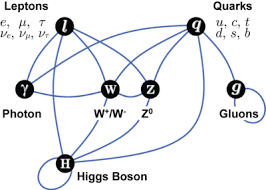
\includegraphics[width=7.0cm,height=6.0cm,scale=0.5]{/home/bibhu/Desktop/PhDThesis/PhDThesis/chapter2/figures2/SMparticlesAndInteractions.png}
    \caption{\small{Summary of the interactions among the SM particles. The plot is taken from Ref.~\cite{SMandParticles}}.}
    \label{fig:standard_modelPart}
\end{figure}


\begin{figure}[h]
    \centering
    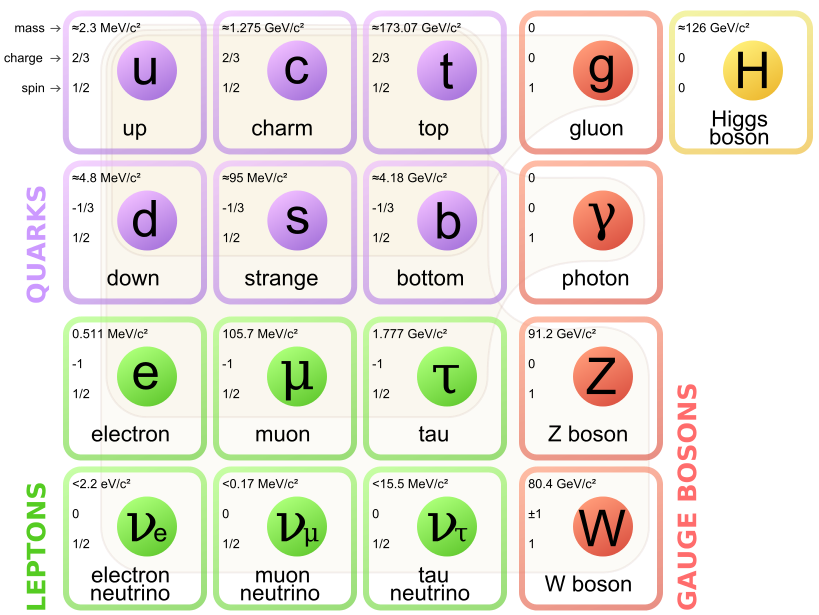
\includegraphics[width=14.0cm,height=10.0cm]{/home/bibhu/Desktop/PhDThesis/PhDThesis/chapter2/figures2/SMparticleProp.png}
    \caption{\small{Masses and other properties of SM particles. The plot is taken from Ref.~\cite{SMandParticles}}}
    \label{fig:SMproperties}
\end{figure}



\begin{table}
\caption{\small{Different interactions and their mediators in nature.}} 
\begin{center}
\begin{tabular}{ | l | l | p{1.5cm}|}
    \hline
     \bf{Interactions} & \bf{Mediators} \\ \hline \hline
     Strong & gluon (g) \\ \hline
     Electromagnetic & photon ($\gamma$) \\ \hline
     Weak & $\rm W^{+}, W^{-}, ~and~ Z^{0}$ \\ \hline 
     Gravitational & graviton (not verified by experiment) \\ \hline
\end {tabular}
\label{Table:Interaction}
\end{center}
\end{table}

	
\section{Gauge Theory Formulation}


The SM is a gauge theory, based on the symmetry group $\rm SU(3)_{C} \otimes SU(2)_{L} \otimes U(1)_{Y}$, which describes strong, weak and electromagnetic interactions,  via the exchange of quanta of the corresponding spin-1 gauge fields. As described earlier, it describes the dynamics of six leptons, six quarks, eight carriers of strong force (gluons), weak vector bosons which mediate the weak interaction, and photon which mediates the electromagnetic interaction. The three families of quarks and leptons are,


$$\left( \begin{array}{cc} u & \nu_{e} \\ d & e  \end{array} \right), \left( \begin{array}{cc} c & \nu_{\mu}  \\ s & \mu  \end{array} \right),\left( \begin{array}{cc} t & \nu_{\tau} \\ b & \tau  \end{array} \right)$$

where each quark appears in three different colors and each particle has its antiparticle. The part of the lagrangian that describes the dynamics of strong force is described by the symmetry group $\rm SU(3)_{C}$(the subscript C stands for color). We call this part as the quantum chromodynamics(QCD) sector. The $\rm SU(3)_{C}$ invariant QCD lagrangian is given by 

\begin{align} \label{LQCD}
\it L_{\rm QCD} &= - \frac{1}{4} G^{\mu\nu}_{a}G^{a}_{\mu\nu} + \sum_{f} \bar{q}_{f} (i\gamma^{\mu}D_{\mu}- m_{f})q_{f},  
\end{align}

where $\it f$ runs over the quark flavors, $\it a$ denotes the summation over eight gluons and $q_{f}$ represents the quark field.  $G^{\mu\nu}_{a}$ is defined as $G^{\mu\nu}_{a}(x) = \del^{\mu}G^{\nu}_{a} - \del^{\nu}G^{\mu}_{a} - g_{s}f^{abc}G^{\mu}_{b}G^{\nu}_{c} $ with $G^{\mu}_{a}$ being the gauge fields. $D^{\mu} = \del^{\mu} + ig_{s}\frac{\lambda^{a}}{2}G^{\mu}_{a}(x)$ and  is  the covariant derivative term, where  $\lambda^{a}$ are the generators of the $\rm SU(3)_{C}$
algebra. All interactions are expressed in terms of a single universal coupling $g_{s}$ which we call the strong coupling constant. The types of interactions between quarks and gluons are followed from the above lagrangian. A large body of experimental evidences for QCD has been gathered over the years. The first evidence for quarks as real constituent elements of hadrons was obtained in deep inelastic scattering experiments at SLAC~\cite{Quark1,Quark2}. The first evidence for gluons came in three jet events at PETRA~\cite{Gluon}.

Two important properties of strong force to be noted are :

{\bf Color confinement~\cite{APichQCD}}, which means that the force between (colored)quarks does not diminish as they are separated. Because of this, when one tries to separate one quark from the other, the energy in the gluon field becomes strong enough to create another quark pair; they are thus forever bound into colorless hadrons such as protons and neutrons. Although analytically unproven, confinement is widely believed to be true as it explains the consistent failure of free quark searches.

{\bf Asymptotic freedom~\cite{APichQCD}}, which means that in very high-energy reactions(few GeV), quarks and gluons interact very weakly creating a quark-gluon plasma. This prediction of QCD was first proposed in the early 1970s by David Politzer, Frank Wilczek and David Gross~\cite{AsympQCD1, AsympQCD2}. 





\section{Electroweak Theory and Higgs Mechanism}

Electroweak theory is a unified theory of electromagnetic and weak interactions. It is described by the symmetry group $\rm SU(2)_{L} \otimes U(1)_{Y}$. The formulation of this theory takes into account a plethora of experimental observations that have been gathered over years. Parity symmetry is known to be maximally violated in weak interactions. This essentially means that the vector bosons do not interact with right-handed fermions, necessitating different representations within the gauge group for different chiral components.  To successfully describe  weak interactions, with several fermionic  flavors and different properties for left- and right-handed fields, and with the requirement that the left-handed fermions should appear in doublets and  we need massive gauge  bosons and massless photon. The simplest group with doublet representations is $\rm SU(2)$. To that we need to include also the electromagnetic interactions necessitating the introduction of an additional group. The symmetry group to consider is then $\rm G = SU(2)_{L}\otimes U(1)_{Y}$, where $\rm L$ refers to left-handed fields and $\rm Y$ denotes hypercharge. We shall come back this later in the chapter. For time being let us introduce the left- and right-handed quark fields as

\begin{align} \label{LRstates}
\rm \psi_{1}(x) &= \left( \begin{array}{cc} u  \\ d  \end{array} \right)_{L},  & \psi_{2}(x) &= u_{R},   & \psi_{3}(x) &= d_{R}.
\end{align}

We will treat the leptons in an identical fashion. The free lagrangian in terms of these fields would be 
\begin{align} \label{L0}
\rm L_{0} &= \sum_{i=1}^{3} i\bar{\psi}_{i}(x)\gamma^{\mu}\del_{\mu}\psi_{i}(x).
\end{align}



 $\rm L_{0}$ is invariant under global G transformations in flavor space:

$\rm \psi_{1}(x) \rightarrow \psi_{1}^{'}(x) = e^{iy_{1}\beta} U_{L} \psi_{1}(x)$ 

$\rm \psi_{2}(x) \rightarrow \psi_{2}^{'}(x) = e^{iy_{2}\beta} \psi_{2}(x)$

$\rm \psi_{3}(x) \rightarrow \psi_{3}^{'}(x) = e^{iy_{3}\beta}  \psi_{3}(x)$

where the $\rm SU(2)_{L}$ transformation $\rm U_{L} = e^{i\frac{\sigma^{i}}{2}\alpha^{i}}$ $\rm (i = 1, 2, 3)$ and $y_{i}$ are hypercharges. If we require the Lagrangian to be invariant under local gauge transformations we will need to introduce covariant derivatives in the following way

$\rm D_{\mu} \psi_{1}(x) = [\del_{\mu} + ig\bar{W_{\mu}}(x) + ig^{'}y_{1}B_{\mu}(x)] \psi_{1}(x)$

$\rm D_{\mu} \psi_{2}(x) = [\del_{\mu} + ig^{'}y_{2}B_{\mu}(x)] \psi_{2}(x)$

$\rm D_{\mu} \psi_{3}(x) = [\del_{\mu} +  ig^{'}y_{2}B_{\mu}(x)] \psi_{3}(x)$

where $\bar{\rm W_{\mu}} = \frac{\sigma^{i}}{2} \rm W^{i}_{\mu}(x)$. There are four different gauge fields, three $\rm W^{i}_{\mu}(x)$s and one $\rm B_{\mu}(x)$ aimed to describe for four gauge bosons. Now the local gauge invariant Lagrangian would be

$\rm L= \sum_{i=1}^{3} i\bar{\psi}_{i}(x)\gamma^{\mu} D_{\mu} \psi_{i}(x)$. 

We note here that the above Lagrangian is without a mass term as the mass term will break the symmetry as left and right components  have different transformation properties. It also does not have the kinetic term for the gauge fields. In order to write the gauge-invariant kinetic term for the gauge fields, we introduce the gauge field tensors as 

$\rm B_{\mu\nu} = \del_{\mu}B_{\nu} - \del_{\nu}B_{\mu}$  and

$\rm \bar{W}_{\mu\nu} = \del_{\mu}\bar{W_{\nu}} - \del_{\nu}\bar{W_{\mu}} + ig[W_{\mu},W_{\nu}]$ leading to 

$\rm L_{kin} = - \frac{1}{4}B_{\mu\nu}B^{\mu\nu} - \frac{1}{4}W_{\mu\nu}^{i}W^{\mu\nu}_{i}$

So the total electroweak Lagrangian is given by
$\rm L_{tot} = L + L_{kin}$. Still the Lagrangian does not have mass terms for the bosons and fermions. In order to accomplish that we will have to break the symmetry of the lagrangian, so that the gauge bosons ($\it W^{+}, W^{-}, Z$) become massive and the photon remains massless.    

In the quantum field theory, a symmetry is `spontaneously' broken when the Lagrangian itself remains invariant with the Hamiltonian of the theory attaining its minimum. In the context of the electroweak theory, spontaneous symmetry breaking is achieved through the introduction of a complex scalar field which attains a nonzero vacuum expectation value (VEV)~\cite{higgs}.

Let us first consider a complex scalar field $\phi(x)$ and the  lagrangian  
\begin{align}\label{Lagra}
\it L & = (\del_{\mu}\phi^{\dagger})(\del^{\mu}\phi) - V(\phi)  \\
V(\phi) & = \mu^{2}\phi^{\dagger}\phi + h(\phi^{\dagger}\phi)^{2}
\end{align}

L is invariant under the global phase transformation of the scalar field. The type of minima of the lagrangian will be different depending on the value of $\mu$. We can have two cases here 
\begin{itemize}
\item $\mu^{2} > 0$, for this the potential has trivial minimum and it describes a massive scalar particle with mass $\mu$ and quartic coupling $h$

\item $\mu^{2} < 0$, in this scenario the minimum of the field is given by  

$|\phi_{0}| = \sqrt{\frac{-\mu^{2}}{2h}}$ $\equiv$ $\frac{v}{\sqrt{2}} > 0$  or $V(\phi_{0}) = -\frac{h}{4}v^{4}$.  Now there are infinite states of degenerate states of minimum energy with solutions given by $\phi_{0} = \frac{v}{\sqrt{2}} e^{i\theta}$. If we choose $\theta =0$ , the symmetry gets spontaneously broken. Now parameterizing the excitations over the ground state as

\end{itemize}

 

$\phi(x) \equiv \frac{1}{\sqrt{2}}[v+\varphi_{1}(x)+ \varphi_{2}(x)]$, where $\varphi_{1}$ and $\varphi_{2}$ are real fields, the potential takes the form 
\begin{align} \label{VafterPar}
\it V(\phi) = V(\phi_{0}) - \mu^{2}\varphi_{1}^{2} + hv\varphi_{1}(\varphi_{1}^{2} + \varphi_{2}^{2}) + \frac{h}{4}(\varphi_{1}^{2} + \varphi_{2}^{2})^{2}
\end{align}


Here $\varphi_{1}$ describes a massive particle with mass $-2\mu^{2}$ and $\varphi_{2}$ is massless. These bosons are called goldstone bosons. In fact, this is quite general result and follows from the Goldstone theorem~\cite{GSW}. At first look, the Goldstone theorem does little to our mass problem. But the problem could be solved through somewhat related mechanism called the Higgs mechanism~\cite{higgs, FR}.


\subsection{Higgs Mechanism}
To discuss the Higgs mechanism, let us consider an $\rm SU(2)_{L}$ doublet of complex scalar fields

\begin{equation} \label{eq1}
\it \phi(x) = \left( \begin{array}{cc} \phi^{(+)}(x)  \\ \phi^{(0)}(x)  \end{array} \right)_{L}
\end{equation}

 Now the gauge invariant lagrangian   becomes 

\begin{equation} \label{eq2HM}
\it L_{S} = (D_{\mu}\phi)^{\dagger} D_{\mu}\phi - \mu^{2}\phi^{\dagger}\phi - h(\phi^{\dagger}\phi)^{2} 
\end{equation}

is invariant under local gauge transformations. Here
 
\begin{equation} \label{eq3HM}
\it D^{\mu}\phi =  [\del^{\mu} + ig\bar{W^{\mu}} + ig^{'}y_{\phi}B^{\mu}]\phi 
\end{equation}

with the vacuum expectation value of $\phi^{0}$ is given by

\begin{equation} \label{VEVHM}
\it {\rm VEV}(\phi^{0}) = \sqrt{\frac{-\mu^{2}}{2h}} \equiv \frac{v}{\sqrt{2}} 
\end{equation}


Once we choose a particular ground state the symmetry gets spontaneously broken. According to the Goldstone theorem, the mass of three massless states will appear. Now parameterizing the scalar doublet in the general form 

\begin{equation} \label{eq4HM}
\it \phi(x) = e^{i\frac{\sigma_{i}}{2}\theta^{i}(x)}\frac{1}{\sqrt{2}}  \left( \begin{array}{cc} 0  \\ v+H(x)  \end{array} \right)_{L} 
\end{equation}

where $\theta^{i}(x)$ and $H(x)$ are four real fields. Now taking a physical gauge $\theta^{i} = 0$ the kinetic part of the Lagrangian takes the form

\begin{align}\label{kineticTerm}
\it (D_{\mu}\phi)^{\dagger} D_{\mu}\phi \rightarrow \frac{1}{2}(\del_{\mu}H) (\del^{\mu}H) + (v+H)^{2} (\frac{g^{2}}{4}W^{\dagger}_{\mu}W^{\mu} + \frac{g^{2}}{8\cos^{2}(\theta_{W})} Z^{\mu}Z_{\mu}) 
\end{align}


We could see from the above term that the gauge bosons have acquired mass. The relationship of their masses is given by 
\begin{equation} \label{ZmWmRel}
\it M_{Z}\cos(\theta_{W}) = M_{W} =\frac{1}{2}vg
\end{equation} 

This is how the Higgs mechanism is responsible for giving masses to vector bosons. Fermions also get masses by Higgs through Yukawa interactions.%~\cite{APichSM}.

\begin{figure}[H]
    \centering
    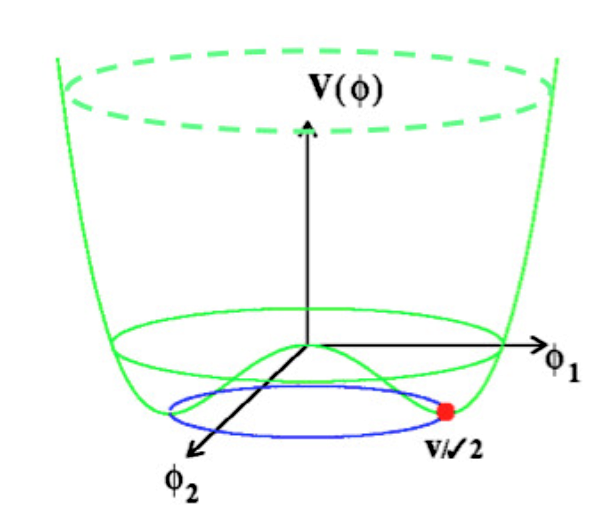
\includegraphics[width=9.0cm,height=6.8cm]{/home/bibhu/Desktop/PhDThesis/PhDThesis/chapter2/figures2/potential.png}
    \caption{ \small {The potential $V(\phi)$ for a complex scalar field $ \phi = \left(\phi_1+ i\phi_2\right)/\sqrt {2}$ where $\mu ^2 < 0$ and $\lambda > 0$ with a minimum at $ v^2 = -\mu^2/\lambda.$ }}
    \label{fig:potential}
\end{figure}

\section {Experimental Verification of SM}

The SM has been phenomenally successful in predicting existence of several particles. All of them have been observed experimentally. The Higgs mechanism has a precise prediction for the $\rm W^{\pm}$ and Z masses, relating them to the vacuum expectation value of the scalar field through Eq(~\ref{ZmWmRel}). It tells $\rm M_{Z}$ should be bigger than $\rm M_{W}$ which is experimentally verified~\cite{WZbosonMass1,WZbosonMass2}.
\begin{equation}\label{WZmass}
M_{Z}  = 91.1875\pm 0.0021 GeV, M_{W} = 80.398\pm 0.025 GeV
\end{equation}

The top quark, being the heaviest one among the known elementary particles, constitutes an important ingredient for precision electroweak tests as well as for an indirect determination of the Higgs boson mass. It was observed for the first time at Tevatron~\cite{topquark}. The recent world-average top mass, driven  LHC measurements is 173.34 $\pm$ 0.27(stat.)$\pm$0.71(syst.)GeV~\cite{TopQuarkMass}.

Another important cornerstone of the SM is the spontaneous electroweak symmetry breaking mechanism proposed almost 50 years ago by Higgs, Brout, Englert,  Guralnik, Hagen and Kibble to generate mass for the  fermions and gauge bosons~\cite{higgs}. This last missing piece to the jigsaw, the Higgs boson, was discovered  by the  CMS~\cite{cms-higgs} and ATLAS~\cite{atlas-higgs} experiments at LHC in 2012. The first observation of the particle was reported in  its high resolution decay channels to $\rm H \rightarrow \gamma\gamma$ and 4-lepton(via $\rm ZZ^{*}$) with a local significance of 5$\sigma$. 



\section {Drawbacks of the Standard Model}

Even though the SM has been very successful in describing many aspects, it cannot be the complete theory due to its inability to explain several experimental observations and mathematical flaws. Some of them can be summarized as below

\begin{itemize}



\item The SM does not explain gravitation. It is unable to successfully marry  theory of gravitation, general relativity with quantum field theory. One of the implications is that plausible quantum field theories of gravity break down before reaching the Planck scale. As a result, we do not have a theory of early universe. 

\item The SM has 19 independent parameters : 9 Yukawa couplings, 3 CKM angles and 1 CP violating phase, 3 coupling constants, the $\mu$ and $\lambda$ parameters of the Higgs potential, and QCD vacuum angle $\theta_{QCD}$ linked to the strong CP problem. It is natural to consider the SM as a low-energy effective theory, far from a fundamental theory.

\item Experiments show neutrinos have mass while the SM does not allow it. In fact, the framework of the SM is based on mass less neutrinos.

\item Dark energy is an unknown form of energy that is hypothesized to permeate all of space, tending to accelerate the expansion of the universe. Several astrophysical observations suggest that universe contains dark matter~\cite{DarkMatter}. The SM does not explain the existence of either dark energy or dark matter.

\item The SM also fails to explain preponderance of matter over antimatter. The CP violation content of the SM falls short by several orders of magnitude in explaining the observed matter-antimatter asymmetry.

\item The Higgs mechanism in the SM gives rise to hierarchy problem, which is, the large discrepancy between the scale of weak interaction and gravity. It is not understood why the former is $\rm 10^{24}$ times stronger than gravity. More technically, why the Higgs boson is so much lighter than the Planck mass. In the context of the SM, the self-energy correction to the Higgs boson mass should diverge.

\end{itemize}





%\end{document}
